\chapter{Models}
\label{cha:models}

Single-Image Super Resolution refers to the process of enhancing the size of small images while striving to minimize the reduction in quality or the loss of detail. Alternatively, it involves the task of reconstructing High Resolution (HR) images by utilizing the abundant information present in Low Resolution (LR) images, which lack finer details.

In other words, Image Super Resolution is about taking images that are of lower quality or resolution and applying techniques to enlarge them without significantly sacrificing their overall quality. This can be particularly useful in scenarios where higher resolution images are required for tasks like printing, displaying on high-resolution screens, or analyzing intricate details in images. The goal is to generate visually appealing results that closely resemble the appearance of true high-resolution images or at least contain improved details compared to the original low-resolution versions.

Neural networks are the perfect tool for this kind of task, from a set of images they are capable of capturing a lot of low-level image statistics and creating powerful high-order models able to deal with a very large degradation space.

The models have been chosen taking into account different characteristics. ESRGAN and Real-ESRGAN are two of the most popular models when it comes to Super Resolution, they share a similar structure and both use a GAN (Generative Adversal Network) architecture, on the other hand, HAT-L and SwinIR are transformer-based models that take a new approach to vision tasks.

All models score highly in the ranking proposed by paperswithcode\cite{pwcode}, which provides a leveled field for comparing the latest models of the most common benchmark datasets.

The four models are implemented in the PyTorch-based open-source image and video restoration toolbox BasicSR (Basic Super Restoration). On top of offering the various models for SR it's equipped with useful logging capabilities and metrics for evaluation.


\section{ESRGAN}
\label{subsec:esrgan}

ESRGAN is based on the SRGAN\cite{ledig2017photorealistic} model. SRGAN, is a generative adversarial network (GAN) for image super-resolution (SR). The SRGAN model uses a perceptual loss function that consists of an adversarial loss and a content loss. The adversarial loss pushes the solution to the natural image manifold using a discriminator network that is trained to differentiate between the super-resolved images and original photo-realistic images. In addition, the authors use a content loss motivated by perceptual similarity instead of similarity in pixel space. The actual networks consist mainly of residual blocks for feature extraction. The perceptual loss function is written as a weighted sum of a VGG content loss and an adversarial loss component. SRGAN is capable of inferring photo-realistic natural images for 4x upscaling factors and is the first framework to achieve this.

\begin{figure}[H]
  \centering
  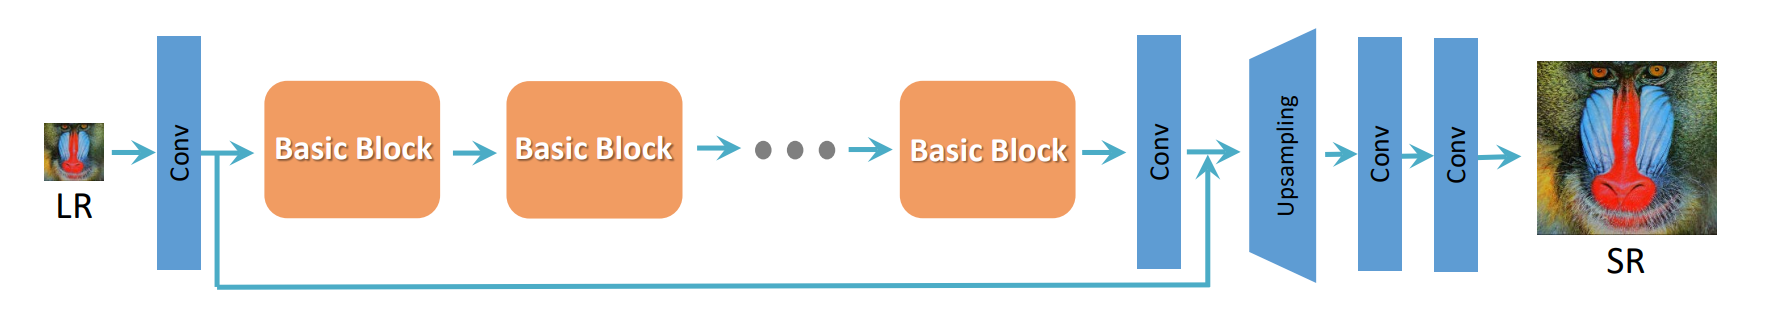
\includegraphics[scale=0.25]{figures/SRResNet.png}
  \caption{The basic architecture of SRResNet.\cite{wang2018esrgan}}
  \label{img:SRResNet}
\end{figure}

ESRGAN stands for Enhanced SRGAN and introduces some major improvements to the framework. The core structure of the network employs an SRResNet architecture (Figure \ref{img:SRResNet}) with two notable differences: the lack of batch normalization and a new structure that replaces the original basic block with the proposed Residual-in-Residual Dense Block (RRDB), which combines multi-level residual network and dense
connections as depicted in Figure \ref{img:RRDB}

\begin{figure}[H]
  \centering
  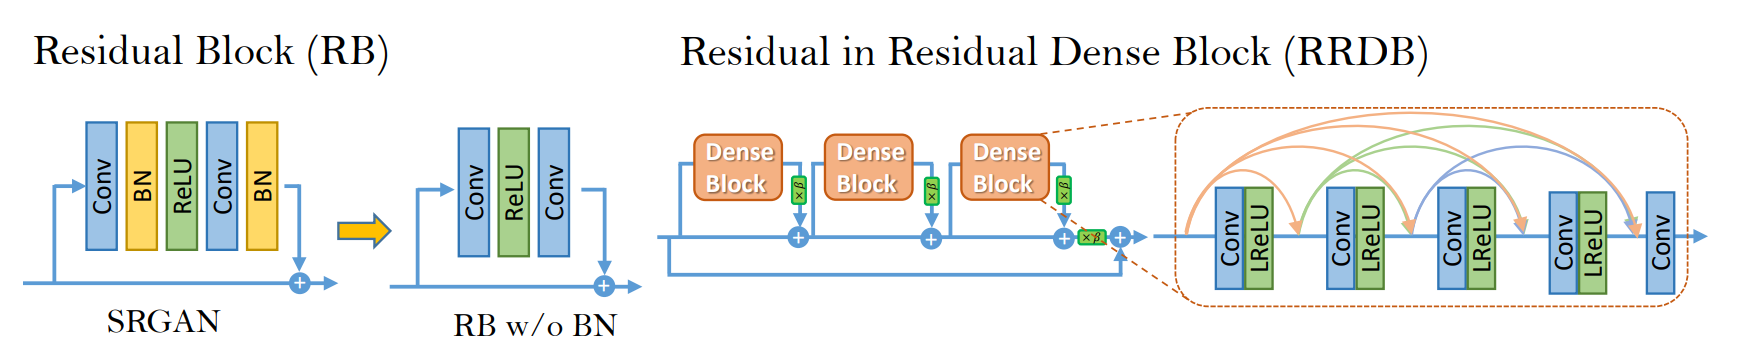
\includegraphics[scale=0.25]{figures/RRDB.png}
  \caption{Left: BN layers removed from residual blocks in SRGAN. Right: RRDB block used in the new deeper model.\cite{wang2018esrgan}}
  \label{img:RRDB}
\end{figure}


\section{Real-ESRGAN}
\label{subsec:realesrgan}

Real-world degradations are usually too complex to be modeled with a simple combination of multiple degradations. Thus, models that assume an ideal bicubic
downsampling kernel or similar degradation processes will easily fail in real-world samples. Real-ESRGAN\cite{9711325} is an expansion of the powerful ESRGAN that introduces a high-order degradation modeling process to better simulate complex real-world degradations, in addition,
it employs a U-Net discriminator with spectral normalization to increase discriminator capability and stabilize the training dynamics.

\begin{figure}[H]
  \centering
  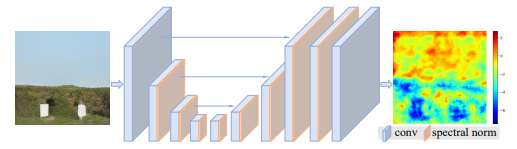
\includegraphics[scale=0.4]{figures/UNET.png}
  \caption{Architecture of the U-Net discriminator.\cite{wang2021realesrgan}}
  \label{img:UNET}
\end{figure}

The authors claim that comparisons have shown superior visual performance than prior works on various real datasets. While in this project the improved degradation model won't help much since our dataset already contains real-world degradations, the improved discriminator and better pratrained weights might yield better results compared to the previous methods.

\section{SwinIR}
\label{subsec:swinir}

CNN-based methods generally suffer from two basic
problems that stem from the basic convolution layer. First, the interactions between images and convolution kernels are content-independent. Using the same convolution kernel to restore different image regions may not be the best choice. Second, under the principle of local processing, convolution is not effective for long-range dependency modeling. As an alternative to CNN, Transformer designs a self-attention mechanism to capture global interactions between contexts and has shown promising performance in several vision problems. However, vision Transformers for image restoration usually divide the input image into patches with fixed size (e.g., 48×48) and process each patch independently. Such a strategy inevitably gives rise to two drawbacks. First, border pixels cannot utilize neighboring pixels that are out of the patch for image restoration. Second, the restored image may introduce border artifacts around each patch. While this problem can be alleviated by patch overlapping, it would introduce an extra computational burden.

More recently Swin Transformer\cite{liu2021swin}  has shown great promise as it integrates the advantages of both CNN and
Transformer. SwinIR\cite{liang2021swinir} is a Swin Transformer-based model that promises impressive performance on high-level vision tasks, such as Super Resolution and Denoising.

\begin{figure}[H]
  \centering
  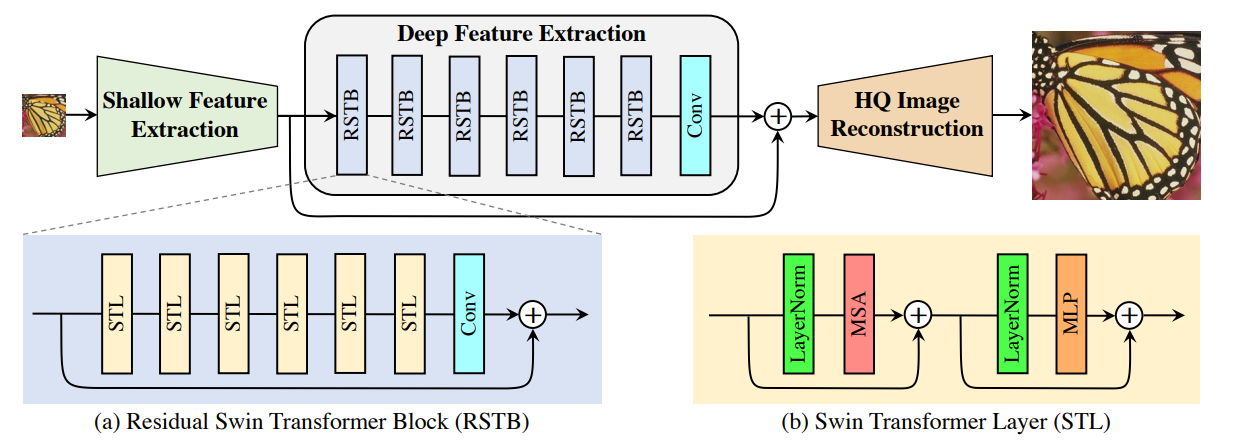
\includegraphics[scale=0.35]{figures/SwinIR.png}
  \caption{Architecture of the SwinIR model with its deep feature extraction module composed of residual Swin Transformer blocks (RSTB).\cite{liang2021swinir}}
  \label{img:swinir}
\end{figure}

\section{HAT-L}
\label{subsec:hatl}

HAT-L expands on the idea of Transformer-based methods for low-level vision tasks, such as image Super Resolution. The authors propose a novel Hybrid Attention Transformer (HAT). It combines both channel attention and window-based self-attention schemes \#TODO expand

\chapter{Training}
\label{cha:Training}

Most of the training has been done using Google Colab Pro on 16GB NVIDIA T4 and NVIDIA V100 GPUs. Due to memory constraints, all models have been trained on the 64 to 256 dataset while only for some it's been possible to use the 128 to 512 dataset.
All trainings were run on pre-trained weights, fine-tuning the model until no improvements could be observed on loss and metrics.

\begin{itemize}
  \item weights for ESRGAN have been pre-trained on  DIV2K\cite{Agustsson_2017_CVPR_Workshops}, Flickr2K\cite{Lim_2017_CVPR_Workshops} and OutdoorSceneTraining\cite{wang2018recovering}. It's been possible to fine-tune the model with all our datasets: 64 to 256, 64 to 256 patches and 128 to 512. For each run, it's been used batch sizes of 4 and 2 and the memory allocated was on average around 7GB for the smaller dataset and 13GB for the bigger one.
  \item Similar to ESRGAN, Real-ESRGAN comes with weights pre-trained on DIV2K, Flickr2K, and OutdoorSceneTraining. The models have been trained on all datasets and, since they share the same generator architecture, the memory allocated was similar to the numbers of ESRGAN.
  \item SwinIR provides weights pre-trained on DIV2K, just like the SRGAN-based models it's been trained on all the dataset configurations with batch sizes of 4 and 2. The memory allocated was around 8GB for the smaller dataset and 14GB for the bigger dataset.
  \item HAT-L proved to be the heaviest of the models. It needed on average 15GB of VRAM just to run the smaller 64 to 256 dataset on a batch size of 2, for this reason, it wasn't possible to try the larger 128 to 512 dataset. The pre-trained weights provided with the model are trained with ImageNet\cite{deng2009imagenet}.
\end{itemize}

\section{Metrics}
\label{sec:metrics}

To evaluate the model performance we used three different metrics: PSNR, SSIM and LPIPS. The first two come integrated into the BasicSR framework and are run at training time during validation, we decided to run additional tests with LPIPS as the powerful metric can in many cases be a better measure of the human eye perception.

\subsection{PSNR}
\label{subsec:psnr}
  PSNR\cite{psnr} stands for "Peak Signal-to-Noise Ratio." It is a metric used to measure the quality of a reconstructed or compressed image or video in comparison to the original, uncompressed version. PSNR is widely used in the field of image and video processing to quantify the level of distortion introduced during compression or transmission.

  The PSNR value is calculated by comparing the maximum possible pixel value (usually 255 for an 8-bit image) to the mean squared error (MSE) between the original and the reconstructed/compressed image. The formula for calculating PSNR is as follows:
  \[
  \text{PSNR} = 10 \cdot \log_{10}\left(\frac{\text{MAX}^2}{\text{MSE}}\right)
  \]

  where \(MAX\) is the maximum possible pixel value and \(MSE\) is the mean squared error between the original and reconstructed images.

\subsection{SSIM}
\label{subsec:ssim}
  The structural similarity index measure (SSIM\cite{ssim}) is a method for predicting the perceived quality of digital images and videos. SSIM is used for measuring the similarity between two images. The SSIM index, just like PSNR, is a full reference metric; in other words, the measurement or prediction of image quality is based on an initial uncompressed or distortion-free image as a reference. The measure between two windows \(x\) and \(y\) of common size \(N \times N\) is:


  \begin{equation}
    \SSIM(x,y) = \frac{(2\mu_x\mu_y + C_1) + (2 \sigma _{xy} + C_2)}
      {(\mu_x^2 + \mu_y^2+C_1) (\sigma_x^2 + \sigma_y^2+C_2)}
    \label{eq:SSMI}
  \end{equation}

  with:
  \begin{itemize}
    \itemsep0em
    \item \(y_x\) the pixel sample mean of \(x\)
    \item \(y_y\) the pixel sample mean of \(y\)
    \item \(\sigma_x^2\) the variance of \(x\)
    \item \(\sigma_y^2\) the variance of \(y\)
    \item \(\sigma _{xy}\) the cross-correlation between \(x\) and \(y\)
    \item \(C_1\) and \(C_2\) two variables to stabilize the division with weak denominator
  \end{itemize}

\subsection{LPIPS}
\label{subsec:LPIPS}
  Perceptual metrics such as PSNR and SSIM, are simple, shallow functions, and fail to account for many nuances of human perception. The deep learning community has found that features
  of the VGG network trained on ImageNet classification has
  been remarkably useful as a training loss for image synthesis \cite{zhang2018unreasonable}, in our specific case the LPIPS (Learned Perceptual Image Patch Similarity) of choice uses the activation layers from AlexNet \cite{NIPS2012_c399862d}


A higher PSNR and SSIM value indicates better image quality, as it signifies a smaller amount of distortion between the original and the processed image. However, it's important to note that while PSNR and SSIM are widely used metrics, it does not always correlate perfectly with human perception of image quality. In some cases, images with higher values might still appear perceptually worse to human observers due to the limitations of the metric in capturing certain types of image distortions that humans are sensitive to. To compensate for this LPIPS provides an excellent estimation of perceptual similarity between images that closely mimics what the human eye can see. A lower LPIPS score means the images are more similar.

\section{Training results}
\label{sec:training_res}

\begin{figure}[H]
  \centering
  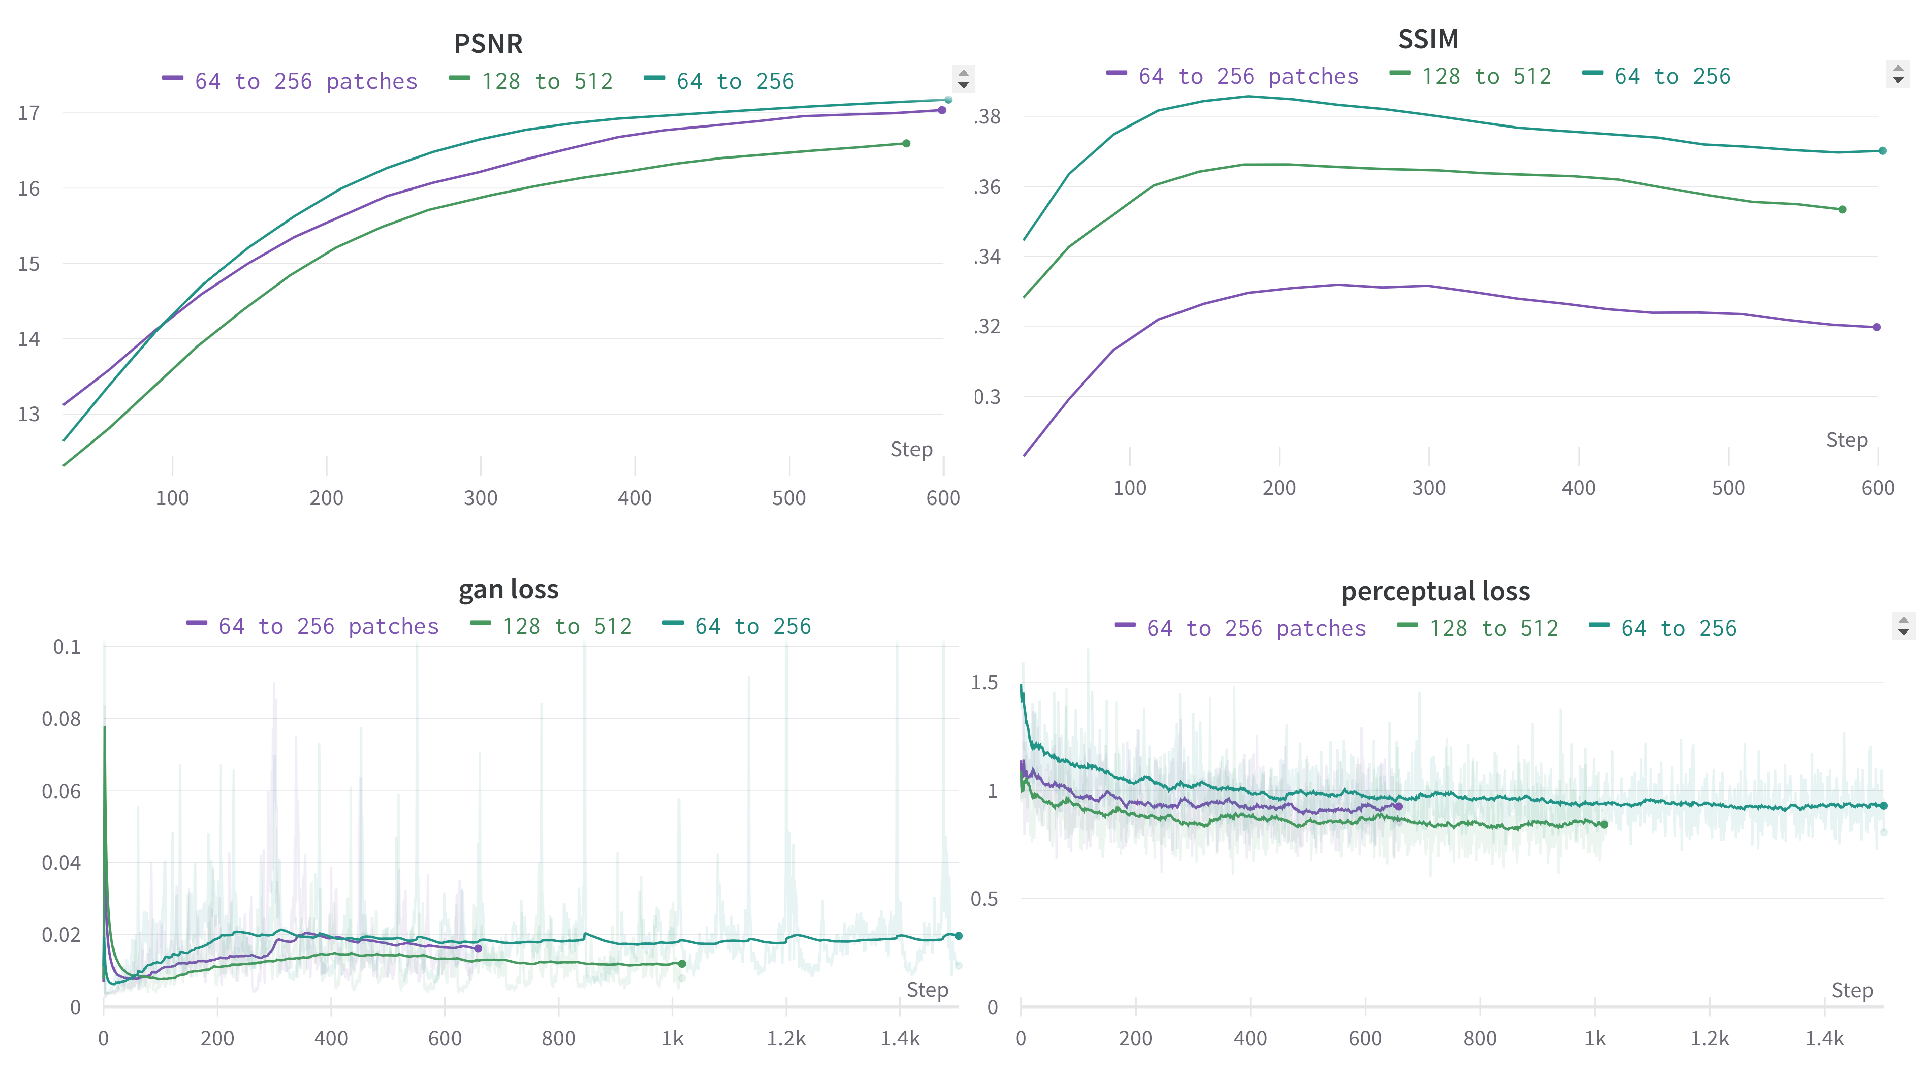
\includegraphics[scale=0.8]{figures/ESRGAN_compose.png}
  \caption{PSNR, SSIM, gan loss and perceptual loss for ESRGAN over the training arch.}
  \label{img:esrgan_training}
\end{figure}

\begin{figure}[H]
  \centering
  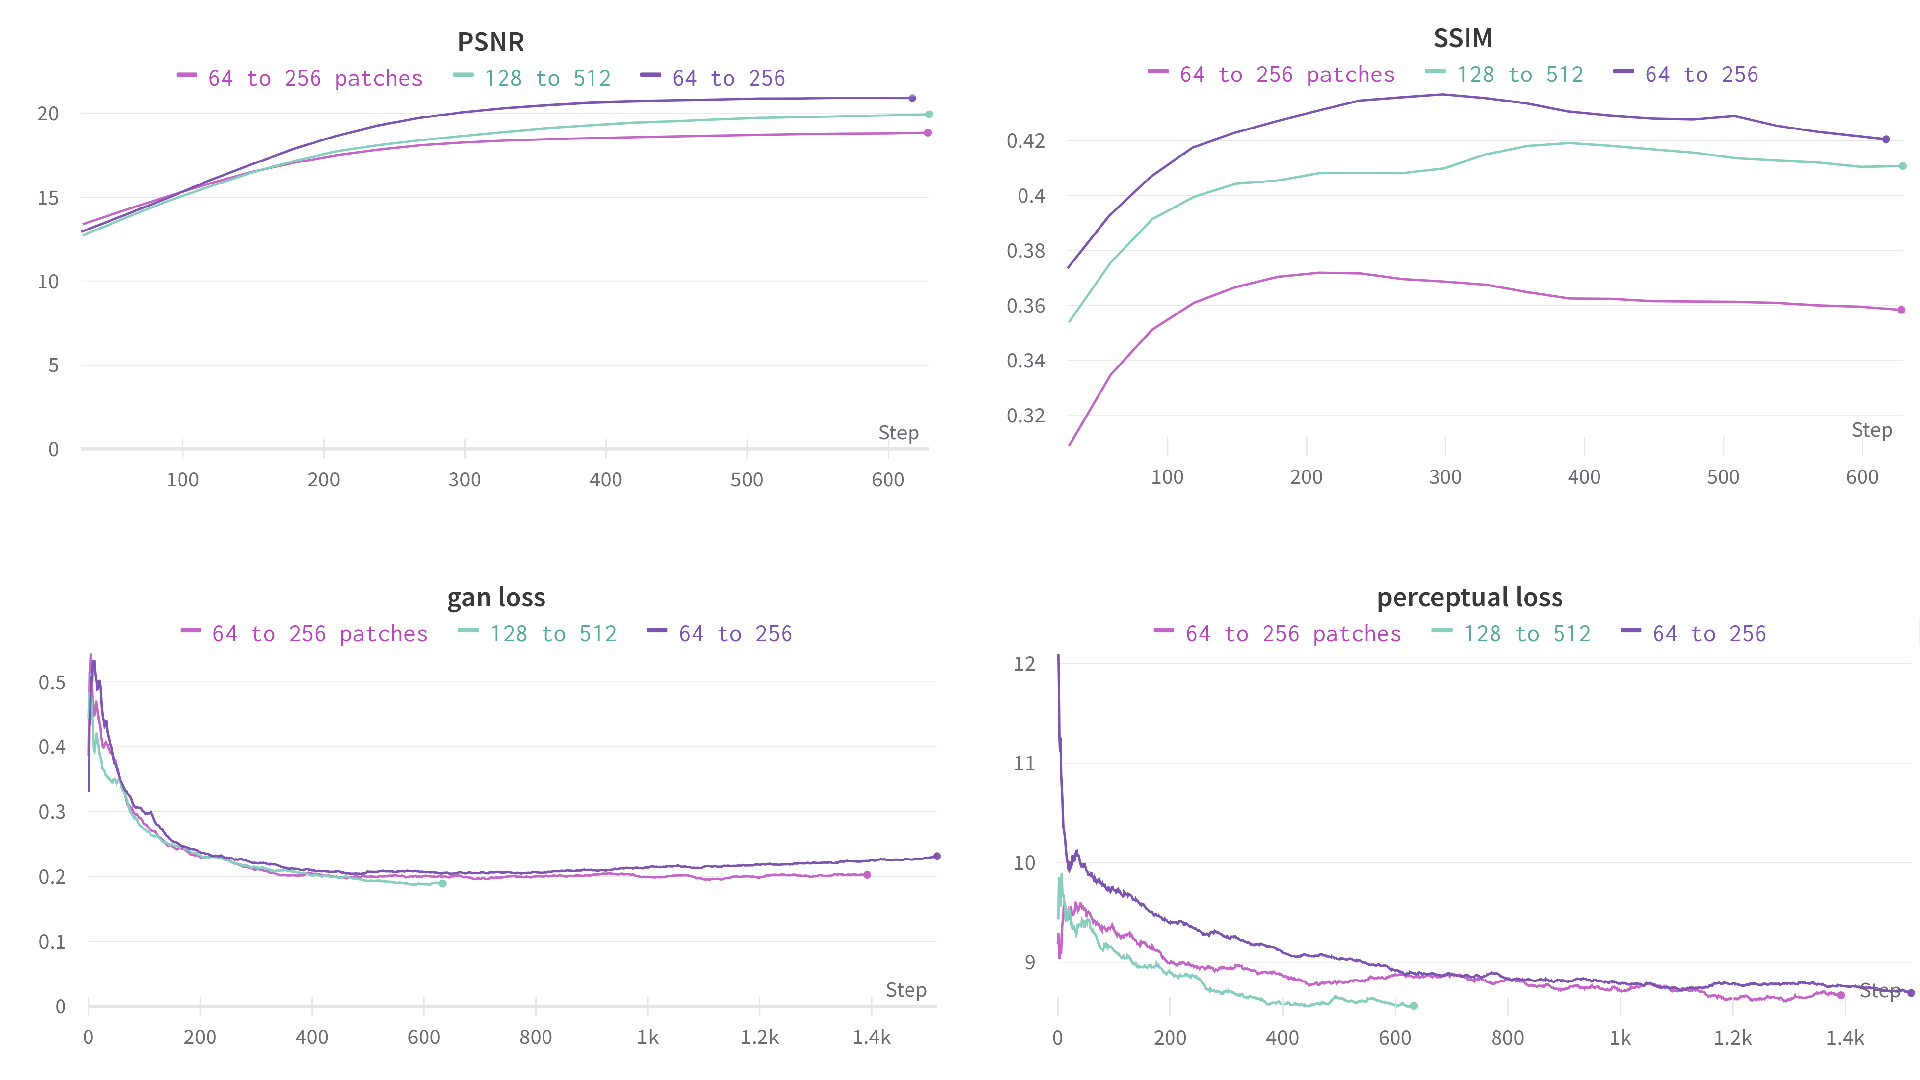
\includegraphics[scale=0.8]{figures/RealESRGAN_compose.png}
  \caption{PSNR, SSIM, gan loss and perceptual loss for Real-ESRGAN over the training arch.}
  \label{img:realesrgan_training}
\end{figure}

\begin{figure}[H]
  \centering
  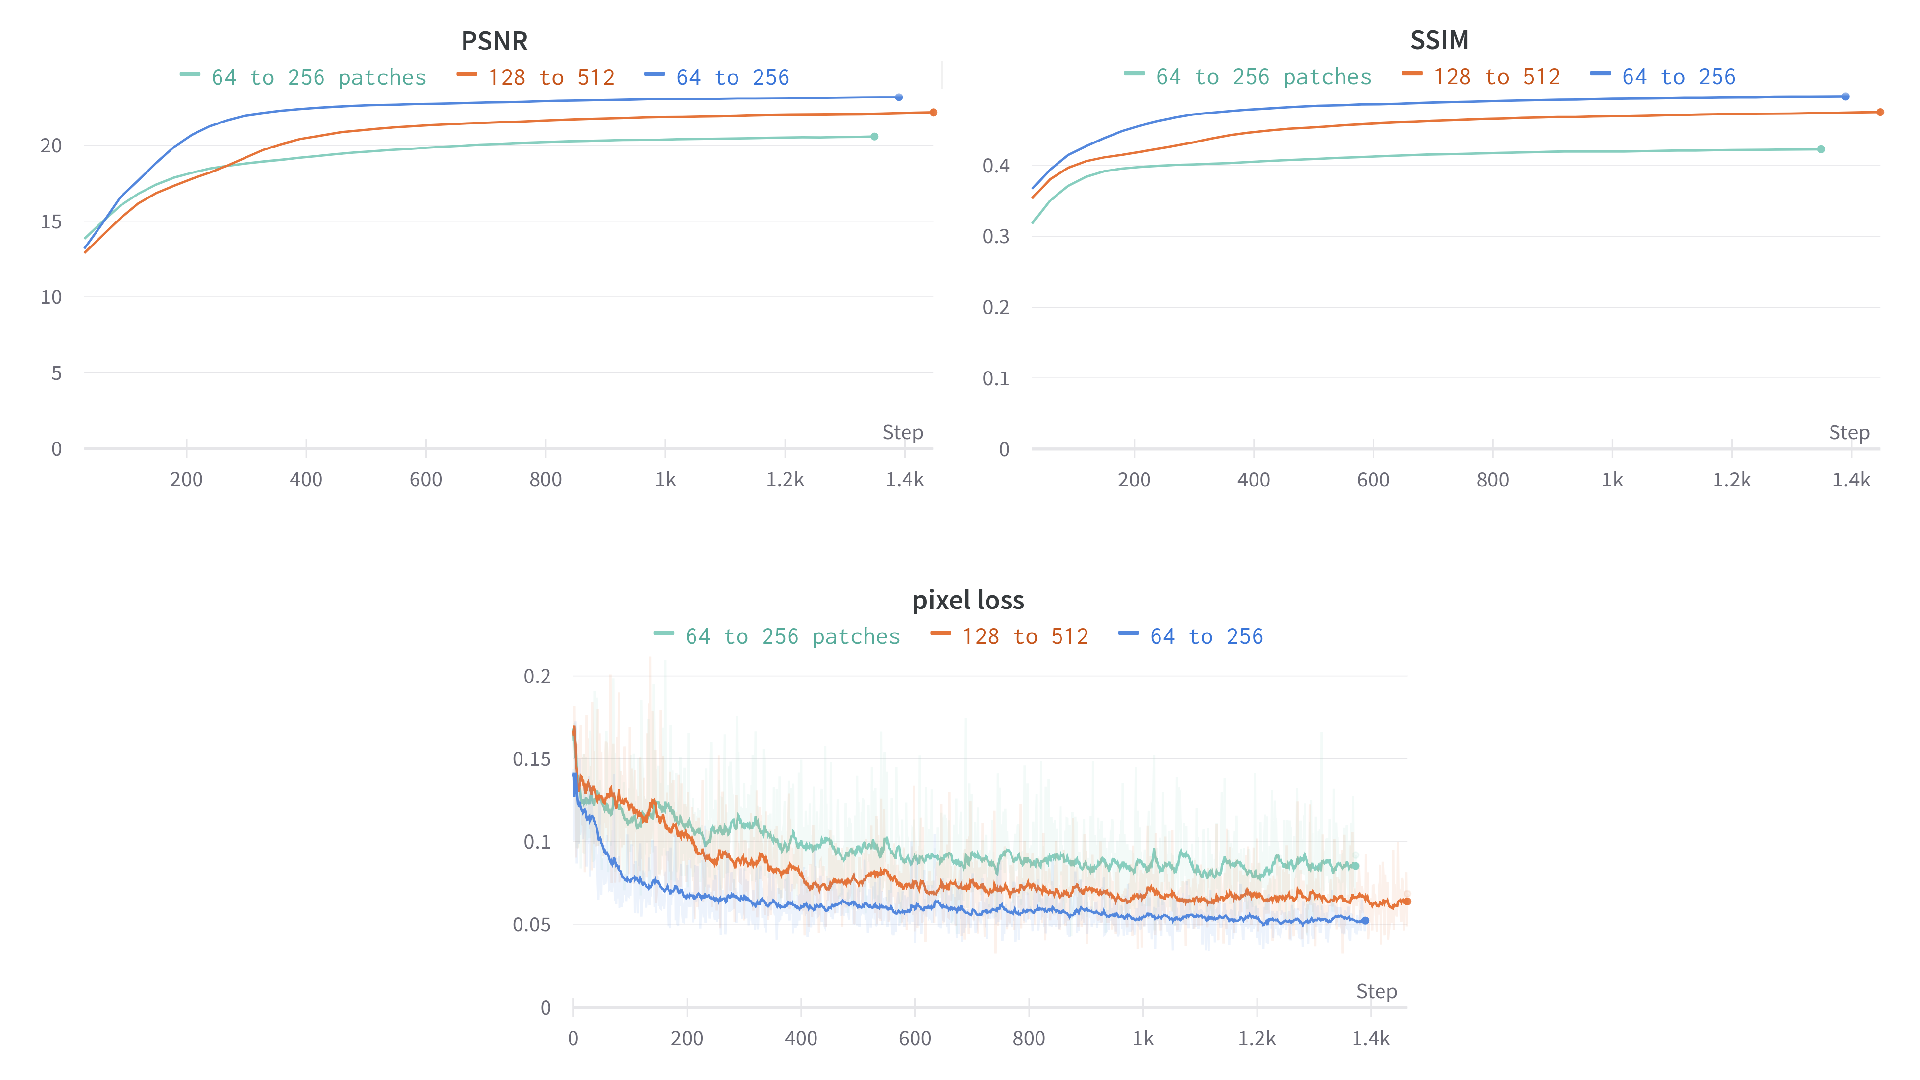
\includegraphics[scale=0.8]{figures/SwinIR_compose.png}
  \caption{PSNR, SSIM and loss for SwinIR over the training arch.}
  \label{img:swinir_training}
\end{figure}

\begin{figure}[H]
  \centering
  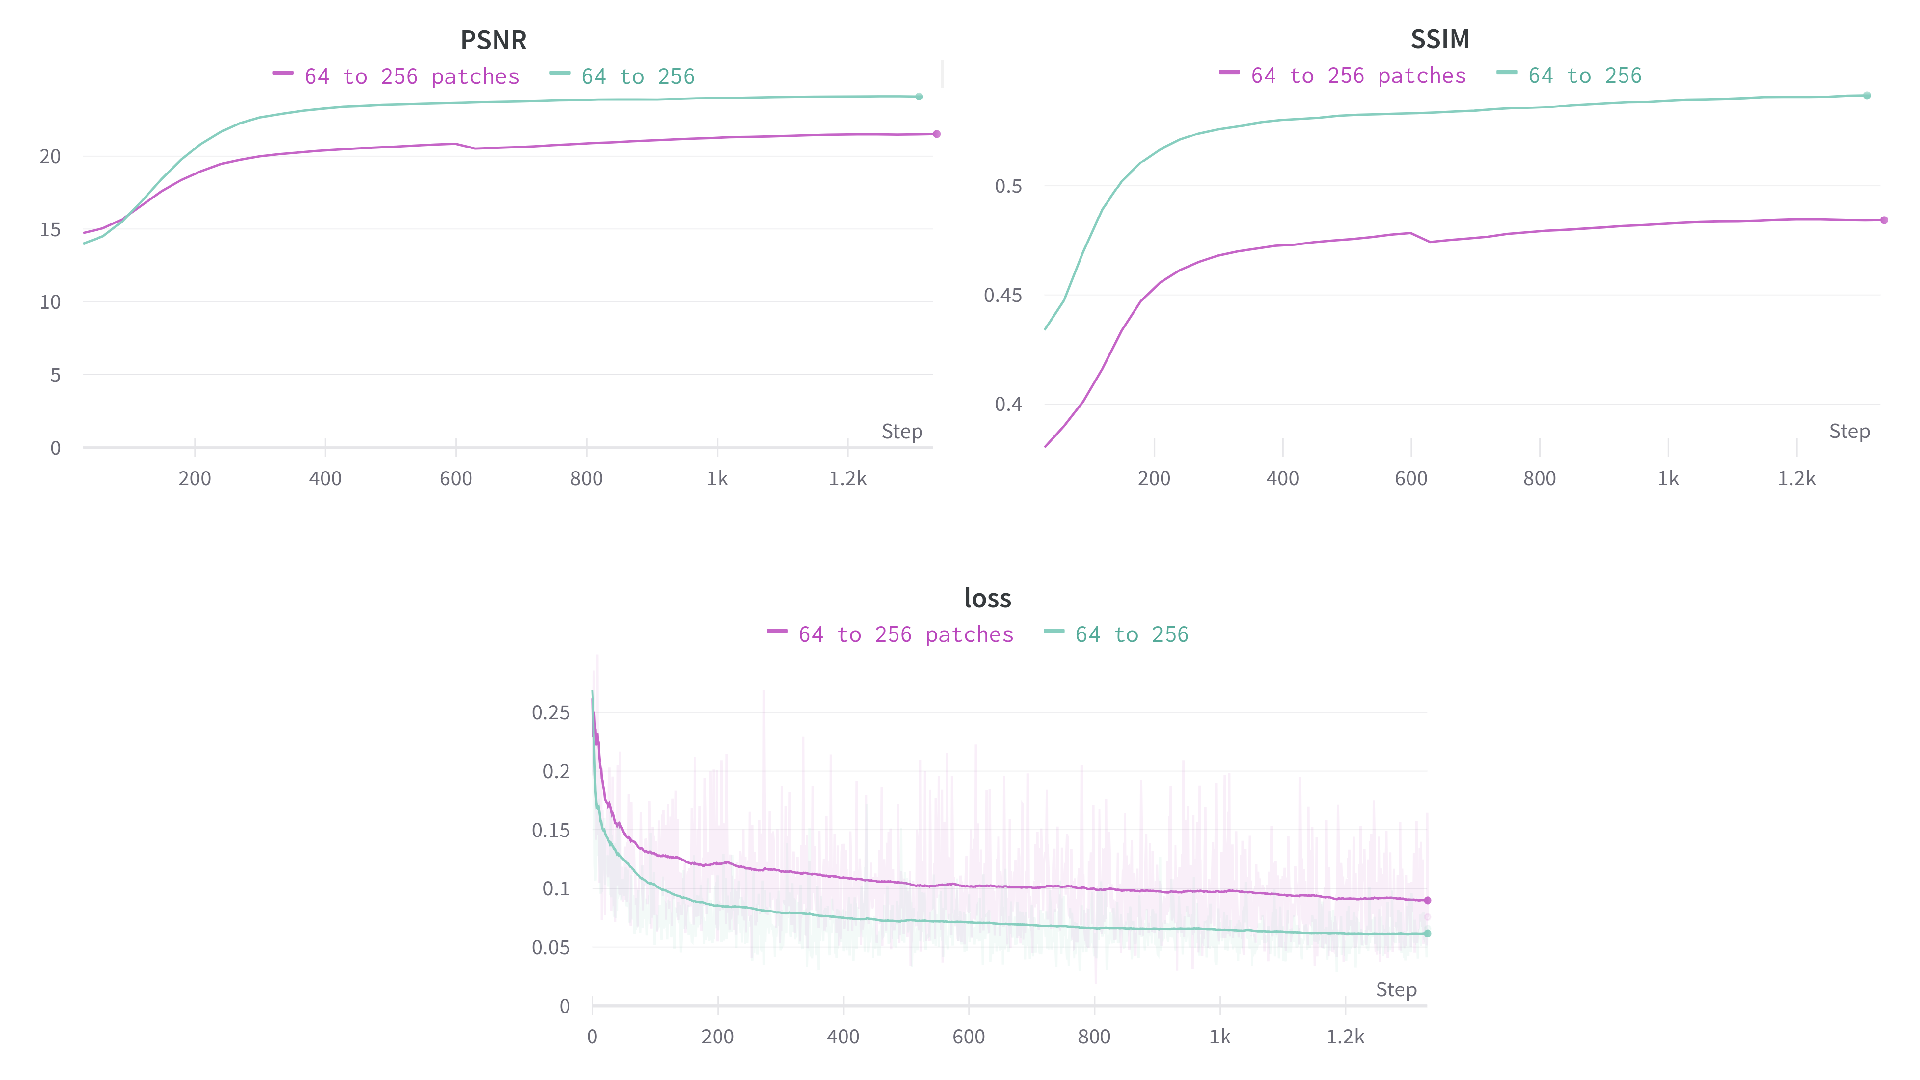
\includegraphics[scale=0.8]{figures/HATL_compose.png}
  \caption{PSNR, SSIM and loss for HAT-L over the training arch.}
  \label{img:hat_training}
\end{figure}

The models have been trained for up to 16k iterations (1 step equals 10 iterations), however from the graphs it's clear that in most cases that was much more than needed. ESRGAN and Real-ESRGAN show similar behavior, with PSNR steadily increasing and SSIM decreasing after around 2k to 3k iterations. HAT-L and SwinIR also had similar behaviours plateauing at around 5k iterations with results definitely better than their GAN-based counterparts. At first glance, the transformer-based model performed much better compared to the others, but the real surprise comes when checking the perceptual similarity metrics.

\begin{figure}[H]
  \centering
  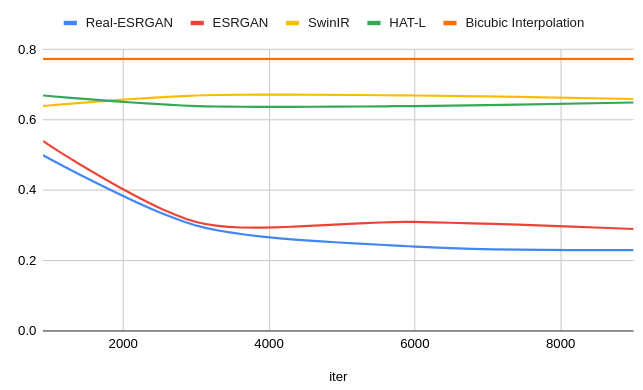
\includegraphics[scale=0.4]{figures/LPIPS_2.png}
  \caption{Comparisons of LPIPS metrics across bicubic interpolation and all models trained on the 64 to 256 dataset (lower is better).}
  \label{img:lpips}
\end{figure}


The disparity in performance between HAT-L and SwinIR, as opposed to Real-ESRGAN and the even more dated ESRGAN, is truly surprising when taking into account the much higher results scored by HAT-L and SwinIR in SSIM and PSNR. This phenomenon is evident in Figure \ref{img:lpips}, notably, the transformer-based models, HAT-L and SwinIR, exhibit a deteriorating trend in perceptual similarity over their training duration, in stark contrast ESRGAN and Real-ESRGAN show constant improvements for the entire arch of training. Table \ref{tab:metrics} provides a comprehensive array of metrics, offering a more comprehensive understanding of the models' performances. This analysis includes Bicubic Interpolation as a baseline, serving as a reference point.


\begin{table}[H]
  \caption{Evaluated metrics for each combination of model and dataset, highlighted in red are the best results and in blue the second best. Bicubic interpolation is added as a baseline.}
  \label{tab:metrics}
  \begin{tabular}{c|ccc|ccc|ccc|}
  \cline{2-10}
  \rowcolor[HTML]{C0C0C0}
  \cellcolor[HTML]{FFFFFF}                                                                       & \multicolumn{3}{c|}{\cellcolor[HTML]{C0C0C0}\textbf{64 to 256}}                                                                                        & \multicolumn{3}{c|}{\cellcolor[HTML]{C0C0C0}\textbf{64 to 256 patches}}                                                                                & \multicolumn{3}{c|}{\cellcolor[HTML]{C0C0C0}\textbf{128 to 512}}                                                                                       \\ \hline
  \rowcolor[HTML]{C0C0C0}
  \multicolumn{1}{|c|}{\cellcolor[HTML]{C0C0C0}\textbf{Model}}                                   & \multicolumn{1}{c|}{\cellcolor[HTML]{C0C0C0}\textbf{PSNR}} & \multicolumn{1}{c|}{\cellcolor[HTML]{C0C0C0}\textbf{SSIM}} & \textbf{LPIPS}               & \multicolumn{1}{c|}{\cellcolor[HTML]{C0C0C0}\textbf{PSNR}} & \multicolumn{1}{c|}{\cellcolor[HTML]{C0C0C0}\textbf{SSIM}} & \textbf{LPIPS}               & \multicolumn{1}{c|}{\cellcolor[HTML]{C0C0C0}\textbf{PSNR}} & \multicolumn{1}{c|}{\cellcolor[HTML]{C0C0C0}\textbf{SSIM}} & \textbf{LPIPS}               \\ \hline
  \multicolumn{1}{|c|}{\textbf{ESRGAN}}                                                          & \multicolumn{1}{c|}{16.981}                                & \multicolumn{1}{c|}{0.369}                                 & {\color[HTML]{3531FF} 0.288} & \multicolumn{1}{c|}{16.328}                                & \multicolumn{1}{c|}{0.317}                                 & {\color[HTML]{3531FF} 0.361} & \multicolumn{1}{c|}{16.34}                                 & \multicolumn{1}{c|}{0.344}                                 & {\color[HTML]{3531FF} 0.353} \\ \hline
  \multicolumn{1}{|c|}{\textbf{Real-ESRGAN}}                                                     & \multicolumn{1}{c|}{20.392}                                & \multicolumn{1}{c|}{0.408}                                 & {\color[HTML]{FE0000} 0.225} & \multicolumn{1}{c|}{17.761}                                & \multicolumn{1}{c|}{0.355}                                 & {\color[HTML]{FE0000} 0.319} & \multicolumn{1}{c|}{{\color[HTML]{3531FF} 19.436}}         & \multicolumn{1}{c|}{{\color[HTML]{3531FF} 0.408}}          & {\color[HTML]{FE0000} 0.307} \\ \hline
  \multicolumn{1}{|c|}{\textbf{SwinIR}}                                                          & \multicolumn{1}{c|}{{\color[HTML]{FE0000} 22.46}}          & \multicolumn{1}{c|}{{\color[HTML]{FE0000} 0.492}}          & 0.667                        & \multicolumn{1}{c|}{{\color[HTML]{FE0000} 19.18}}          & \multicolumn{1}{c|}{{\color[HTML]{FE0000} 0.417}}          & 0.761                        & \multicolumn{1}{c|}{{\color[HTML]{FE0000} 21.25}}          & \multicolumn{1}{c|}{{\color[HTML]{FE0000} 0.466}}          & 0.696                        \\ \hline
  \multicolumn{1}{|c|}{\textbf{HAT-L}}                                                           & \multicolumn{1}{c|}{{\color[HTML]{3531FF} 21.63}}          & \multicolumn{1}{c|}{{\color[HTML]{3531FF} 0.478}}          & 0.651                        & \multicolumn{1}{c|}{{\color[HTML]{3531FF} 18.71}}          & \multicolumn{1}{c|}{{\color[HTML]{3531FF} 0.409}}          & 0.684                        & \multicolumn{1}{c|}{/}                                     & \multicolumn{1}{c|}{/}                                     & /                            \\ \hline
  \multicolumn{1}{|l|}{\textbf{\begin{tabular}[c]{@{}l@{}}Bicubic\\ Interpolation\end{tabular}}} & \multicolumn{1}{l|}{11.82}                                 & \multicolumn{1}{l|}{0.354}                                 & \multicolumn{1}{l|}{0.774}   & \multicolumn{1}{l|}{11.76}                                 & \multicolumn{1}{l|}{0.287}                                 & \multicolumn{1}{l|}{0.717}   & \multicolumn{1}{l|}{11.71}                                 & \multicolumn{1}{l|}{0.332}                                 & \multicolumn{1}{l|}{0.735}   \\ \hline
  \end{tabular}
  \end{table}

The results in Table \ref{tab:metrics} have been evaluated taking into consideration for each combination of model and dataset the checkpoint with best performance. With that model, each LR image of the validation set has been supersampled and analyzed with its corresponding ground truth. Unlike for the results in Figures \ref{img:esrgan_training}, \ref{img:realesrgan_training}, \ref{img:swinir_training} and \ref{img:hat_training}, the implementation of SSIM and PSNR used is not the one provided directly by BasicSR but we used Torchmetrics' implementation, the LPIPS implementation comes from the original library \cite{lpips2}.

In red and blue are highlighted respectively the best and second-best score for each metric. While SwinIR outperformed all the other models in both PSNR and SSIM and HAT-L comes a close second in the same metrics, Real-ESRGAN and ESRGAN showed the best results overall for perceptual similarity with a good margin on the transformer-based models.


\begin{figure}[H]

  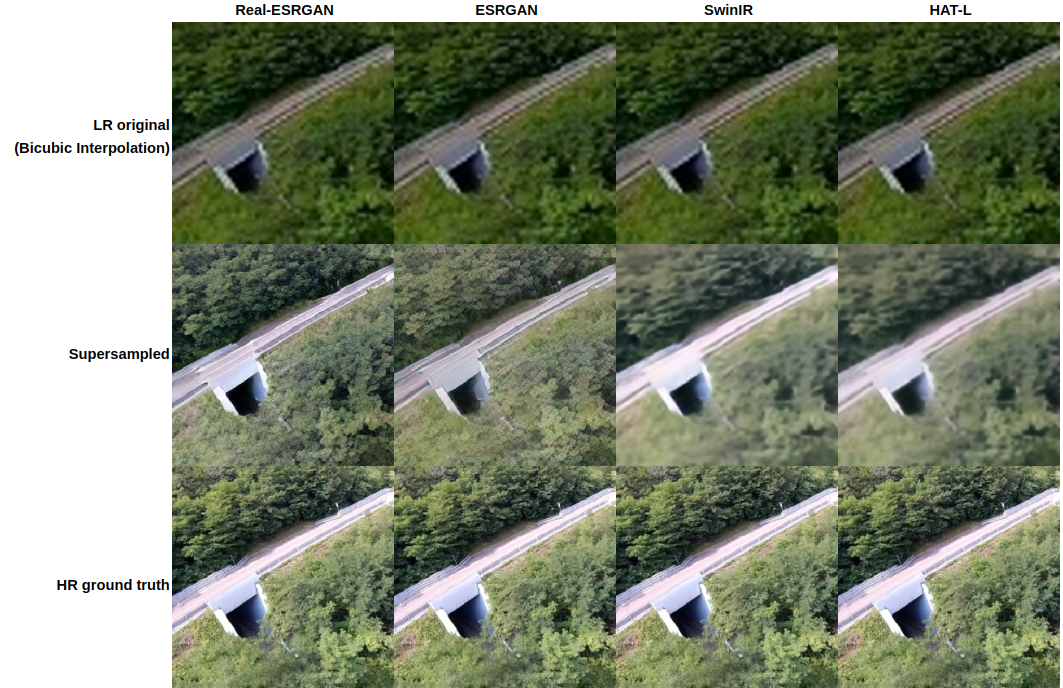
\includegraphics[scale=0.4]{figures/results/comp_table.png}
  \caption{Final results compared side by side.}
  \label{img:comp_table}
\end{figure}

In Figure \ref{img:comp_table} is even clearer the reason for good perceptual similarity results in Real-ESRGAN and ESRGAN: the supersampled images from HAT-L and SwinIR look blurred while the other two are sharp with fine details and defined edges.


\chapter{Results}
\label{cha:Results}
